%!TEX root = ../thesis.tex
%*******************************************************************************
%****************************** Second Chapter *********************************
%*******************************************************************************

\chapter{Background}
\label{chapter2}

\ifpdf
    \graphicspath{{Chapter2/Figs/Raster/}{Chapter2/Figs/PDF/}{Chapter2/Figs/}}
\else
    \graphicspath{{Chapter2/Figs/Vector/}{Chapter2/Figs/}}
\fi

%********************************** %First Section  **************************************
\section{Lattice models}
\label{sec:lattice-models}

\subsection{Historical introduction}
\label{subsec:latt-hist}

\subsection{The Schr{\"o}dinger equation}
\label{subsec:latt-qm}

\subsection{Canonical examples of lattice models}
\label{subsec:latt-examples}

\subsubsection{Quantum Ising model}
\subsubsection{Heisenberg model}
\subsubsection{Bose-Hubbard model}

%********************************** %Second Section  *************************************
\newpage
\section{Quantum Monte Carlo}
\label{sec:qmc}

\subsection{Overview}
\label{subsec:qmc-hist}
%% General about QMC
Quantum Monte Carlo is a class of methods that uses statistical sampling to directly deal with high-dimensional integration that arises from working with the many-body wave function. QMC methods are among the most accurate achieving chemical accuracy for smaller systems~\cite{foulkes2001quantum}, and can achieve any degree of statistical precision sought. Quantum Monte Carlo is also very versatile and can be applied at both zero and finite temperatures~\cite{austin2012quantum}.	
%% Zero temperature methods
%% Variational quantum monte carlo
The most basic zero temperature QMC method is variational QMC (VMC). The method is composed of two parts, firstly it directly evaluates the variational energy $E_V = \langle \Psi_{T} | \hat H | \Psi_{T} \rangle / \langle \Psi_{T} | \Psi_{T} \rangle$ of the system using Monte Carlo integration and a trial wave function $\Psi_{T}$. Secondly the parameters of the trial wave function are optimised such as to minimise the variational energy $E_V$, giving the method its name. The first application of VMC was to ground state ${}^4$He~\cite{mcmillan1965ground} and was later extended for studying many-body fermionic systems~\cite{ceperley1977monte}. A way of obtaining excitation energies using VMC is to use a trial wave function that models an excited state of the system, if the trial wave function obeys a certain symmetry, the variational principle guarantees that this VMC energy calculation gives an upper bound on the lowest exact eigenstate of this symmetry. Furthermore, the method can be extended to study non-equilibrium properties of bosonic~\cite{carleo2012localization, carleo2014light}, and fermionic~\cite{ido2015time} systems. The main advantage of VMC is its simplicity while the main drawback is that the accuracy is limited by the flexibility and form of the trial wave function~\cite{austin2012quantum}. As such VMC is usually employed as a first step in more advanced QMC simulations. 

%% Green function QMC and Diffusion QMC
Projector quantum Monte Carlo (PMC) is a class of QMC methods which are in essence nothing more than stochastic implementations of the power method to obtain the dominant eigenvector of a matrix or a kernel function~\cite{gubernatis_kawashima_werner_2016}. Their distinct advantage over VMC is that they are not constrained by our parametrisation of the trial wave function, as they can describe arbitrary probability distributions. The projector $\hat P$ has to be chosen in such a way, that the ground state of the system becomes the dominant eigenvector, i.e. $| \Psi_{0}\rangle = \lim_{n\rightarrow \infty} \hat{P}^n |\Psi_{T}\rangle$. Different ways of achieving this give rise to different flavours of PMC methods, e.g choice of space (real or orbital space) in which the walk is done and choosing either first or second quantisation. Using an exponential projector $\hat{P} = e^{\tau (E_T \mathbb{1} - \hat{H})}$ can be interpreted as propagation in imaginary time $\tau \rightarrow it$ in turn transforming the Schr\"odinger equation into a diffusion equation, which is a continuous limit of the random walk and lends itself to stochastic integration~\cite{reynolds1990diffusion}. Directly sampling from the exact Green function is known as Projector Green Function Monte Carlo (GFMC) method~\cite{kalos1962monte, kalos1966stochastic}. A convenient approximation to GFMC is its short-time approximation which leads to one of the most popular QMC methods, diffusion Monte Carlo (DMC)~\cite{foulkes2001quantum, reynolds1990diffusion}. In this regime one can exploit analytical solutions to diffusion and rate problems to write an explicit form of the Green's function. Additionally, by using the Trotter-Suzuki formula the time-step bias can be expressed and accounted for~\cite{austin2012quantum}. DMC is statistically implemented by using a population of walkers which either branch or die, over which the average is calculated. Reptation quantum Monte Carlo~\cite{reynolds1990diffusion} (RMC) is an alternative formulation which only uses a single walker, and instead of branching and dying the MC moves mutate the path of that single walker. The use of a guiding wave function for importance sampling greatly improves the statistical efficiency of PMC methods. The guiding wave function is usually obtained by means of VMC or some mean field calculation. 

PMC methods suffer from the \emph{sign problem}, which is present in Markov chain simulation of distributions that are not strictly positive, thus in fermionic and frustrated systems~\cite{gubernatis_kawashima_werner_2016}. The problem refers to an exponential decrease in sampling efficiency with system size. The search for solutions of this problem is still an area of active research~\cite{foulkes2001quantum} but is in practice remedied by the \emph{fixed-node} approximation~\cite{anderson1975random}. It imposes a boundary condition into the projection, such that the projected state shares the same zero crossings (nodal surface) with a trial wave function, which is again usually obtained with VMC. The projected state is now only exact when the nodal surface is exact. Nevertheless this approximation is quite accurate~\cite{foulkes2001quantum}. Fixed node is widely used, one of its first applications being the electron gas~\cite{ceperley1980ground}, which is used in parameterisations of the  exchange correlation functional in LSDA~\cite{vosko1980accurate}.

%% Finite temperature methods
Quantum Monte Carlo methods have had a lot of success at finite temperatures. Auxiliary-field Monte Carlo, or Path Integral Monte Carlo~\cite{ceperley1995path}, which leads to ring-polymer molecular dynamics, may be used for this purpose. Additionally QMC is not limited to continuum space applications and has been extensively used to study lattice models, notable examples being the cluster/loop algorithm and the worm algorithm~\cite{gubernatis_kawashima_werner_2016, prokof1998exact}.

%% Computational considerations
Quantum Monte Carlo methods are generally more computationally expensive than DFT approaches, but on the other hand QMC codes are, as a rule of thumb, simpler to implement. Furthermore, since the wave function does not need to be stored directly, QMC has reasonable storage requirements. The high computational cost of the QMC methods is remedied by the fact that they are intrinsically parallelisable, the core calculation involves generating (pseudo)-random numbers, performing a simple calculation and in the end averaging over the results. Therefore, implementations of QMC algorithms that have been applied to practical problems are optimised to run on massively parallel hardware with little overhead~\cite{needs2020variational}. Finally, the repetitive nature of the Monte Carlo calculation lends itself to hardware acceleration using either graphical processing units (GPUs) or field-programmable gate arrays (FPGAs)~\cite{austin2012quantum}.

\subsection{Implementation}
\label{subsec:qmc-impl}
\subsubsection{Monte Carlo Importance Sampling}
The most common application of Monte Carlo methods is evaluation of integrals in high dimensional space. There MC has a distinct advantage over quadrature methods, as the statistical error decreases with the square root of samples irregardless of the dimensionality of the problem. Integrals of a function $g(\mathbf{R})$
\begin{equation}
	I=\int g(\mathbf{R}) \mathrm{d} \mathbf{R},
\end{equation}
where $\mathbf{R}$ is the \emph{configuration} of the system or simply a \emph{walker}, can be integrated by use of an \emph{importance function} $\mathrm{P}(\mathbf{R})$, where $\int d \mathbf{R} \text{P}(\mathbf{R})=1$ and $\mathrm{P} (\mathbf{R}) \geq 0$. The integral can be rewritten in the form
\begin{equation}
	\int g(\mathbf{R}) \mathrm{d} \mathbf{R} = \int \frac{g(\mathbf{R})}{\mathrm{P}(\mathbf{R})} \mathrm{P}(\mathbf{R}) \mathrm{d} \mathbf{R} = \int f(\mathbf{R})\mathrm{P}(\mathbf{R}) \mathrm{d} \mathbf{R},
\end{equation}
where $f(\mathbf{R}) = g(\mathbf{R}) / \mathrm{P}(\mathbf{R})$.
The importance function $\mathrm{P}(\mathbf{R})$ can be interpreted as a probability density. If we generate an infinite number of random uncorrelated configurations $\mathbf{R}_m$ from the distribution $\mathrm{P}(\mathbf{R})$, the sample average is a good estimator of the integral $I$
\begin{equation}
	I=\lim _{M \rightarrow \infty}\left\{\frac{1}{M} \sum_{m=1}^{M} f\left(\mathbf{R}_{m}\right)\right\},
\end{equation}
and for an approximation with a finite number of samples
\begin{equation}
	I \approx \frac{1}{M} \sum_{m=1}^{M} f\left(\mathbf{R}_{m}\right).
\end{equation}
Under conditions where the central limit theorem holds~\cite{foulkes2001quantum}, the estimator is normally distributed with variance $\sigma_{f}^{2}/M$, which can also be estimated from the samples as
\begin{equation}
	\frac{\sigma_{f}^{2}}{M} \approx \frac{1}{M(M-1)} \sum_{m=1}^{M}\left[f\left(\mathbf{R}_{m}\right)-\frac{1}{M} \sum_{n=1}^{M} f\left(\mathbf{R}_{n}\right)\right]^{2}.
\end{equation}
In the case of Hookium, the configurations $\mathbf{R}$ are the positions of the electrons.

\subsubsection{Metropolis-Hastings algorithm}
The integration technique from the previous section relies on our ability to obtain samples from a probability distribution $\mathrm{P}(\mathbf{R})$. In the case of QMC these distributions are high-dimensional and cannot be directly sampled from. Moreover their normalisations are usually not known. 
The Metropolis-Hastings algorithm~\cite{hastings1970monte}, see Algorithm~1, avoids direct sampling from the distribution $\mathrm{P}(\mathbf{R})$ and is insensitive to its normalisation. It uses a Markov process whose stationary distribution $\pi(\mathbf{R})$ is the same as $\mathrm{P}(\mathbf{R})$	
to generate a sequence of configurations $\left\{\mathbf{R}_n\right\}_\mathrm{P}$ 
that are drawn from $\mathrm{P}(\mathbf{R})$. A Markov process is completely defined with its transition probability $\mathrm{P}(\mathbf{R} \rightarrow \mathbf{R}^\prime)$, which is the probability of transitioning from state $\mathbf{R}$ to state $\mathbf{R}^\prime$. For the process to have a unique stationary distribution two conditions must be met, the process must be \emph{ergodic} and it must obey \emph{detailed balance}
\begin{equation}
	\mathrm{P}(\mathbf{R}) \mathrm P(\mathbf{R} \rightarrow \mathbf{R}^\prime) = \mathrm{P}(\mathbf{R}^\prime) \mathrm P(\mathbf{R}^\prime \rightarrow \mathbf{R}),
\end{equation}
rewritten as
\begin{equation}
	\label{eq:detailed_balance}
	\frac{\mathrm P ({\mathbf{R}})}{\mathrm P ({\mathbf{R}^\prime})} = \frac{\mathrm P(\mathbf{R}^\prime \rightarrow \mathbf{R})}{\mathrm P(\mathbf{R} \rightarrow \mathbf{R}^\prime)}.
\end{equation}
The right transition probability $\mathrm P(\mathbf{R} \rightarrow \mathbf{R}^\prime)$ is not known, but we can express it with a trial move transition probability $\mathrm{T}(\mathbf{R} \rightarrow \mathbf{R}^\prime)$ which we sample and acceptance probability $\mathrm{A}(\mathbf{R} \rightarrow \mathbf{R}^\prime)$ as
\begin{equation}
	\mathrm P(\mathbf{R} \rightarrow \mathbf{R}^\prime) = \mathrm T(\mathbf{R} \rightarrow \mathbf{R}^\prime) \mathrm A(\mathbf{R} \rightarrow \mathbf{R}^\prime).
\end{equation}
For equation~\eqref{eq:detailed_balance} to hold, the acceptance probability must be 
\begin{equation}
	A\left(\mathbf{R} \rightarrow \mathbf{R}^{\prime}\right)=\min \left(1, \frac{\mathrm{T}\left(\mathbf{R}^{\prime} \rightarrow \mathbf{R}\right) \mathrm{P}\left(\mathbf{R}^{\prime}\right)}{\mathrm{T}\left(\mathbf{R} \rightarrow \mathbf{R}^{\prime}\right) \mathrm{P}(\mathbf{R})}\right).
\end{equation}
Thus to sample from any probability distribution we need only have the ability to calculate probabilities $\mathrm P(\mathbf{R})$ and to sample from a trial transition probability $\mathrm T(\mathbf{R} \rightarrow \mathbf{R}^{\prime})$. The efficiency of the algorithm depends on the amount of trial moves that we reject. All trial moves would be accepted if $\mathrm{T}(\mathbf{R} \rightarrow \mathbf{R}^{\prime})= \mathrm{P}(\mathbf{R}^\prime)$, which would just mean sampling from $\mathrm P$ directly and is the very problem we are trying to solve with Metropolis-Hastings. 	
\begin{algorithm}
	\label{alg:MCMC}
	\SetAlgoLined
	\KwResult{A set of configurations $\left\{ \mathbf{R}_n \right\}_{\mathrm{P}}$ sampled from $\mathrm P$}
	Initialize walker at random configuration $\mathbf{R}$\;
	\While{no. samples less than $N$}{
		Generate new configuration $\mathbf{R}^\prime$ with transition probability $\mathrm{T}(\mathbf{R}\rightarrow\mathbf{R}^\prime)$\;
		
		Accept the move ($\mathbf{R} \rightarrow \mathbf{R}^\prime$) with probability $A\left(\mathbf{R} \rightarrow \mathbf{R}^{\prime}\right)=\min \left(1, \frac{\mathrm{T}\left(\mathbf{R}^{\prime} \rightarrow \mathbf{R}\right) \mathrm{P}\left(\mathbf{R}^{\prime}\right)}{\mathrm{T}\left(\mathbf{R} \rightarrow \mathbf{R}^{\prime}\right) \mathrm{P}(\mathbf{R})}\right)$\;
		
		Append $\mathbf{R}$ to the set of configuration;
		
	}
	\caption{Metropolis-Hastings}
\end{algorithm}

\subsubsection{Variational Quantum Monte Carlo}
Variational quantum Monte Carlo uses a trial wave function $\Psi_{T}$ which is an approximation to the true ground state wave function to directly evaluate the expectation value of $\hat H$. This provides an upper bound on the ground state energy
\begin{equation}
	\label{eq:variational_princ}
	E_{V}=\frac{\langle \Psi_{T} | H | \Psi_{T} \rangle}{\langle \Psi_{T} | \Psi_{T} \rangle}
	=\frac{\int \Psi_{T}^{*}(\mathbf{R}) \hat{H} \Psi_{T}(\mathbf{R}) d \mathbf{R}}{\int \Psi_{T}^{*}(\mathbf{R}) \Psi_{T}(\mathbf{R}) d \mathbf{R}} \geq E_{0}.
\end{equation}
The expression for the variational energy $E_V$ can be rewritten as
\begin{equation}
	\label{eq:E_V}
	E_{V}=\frac{\int\left|\Psi_{T}(\mathbf{R})\right|^{2}\left(\Psi_{T}(\mathbf{R})^{-1} \hat{H} \Psi_{T}(\mathbf{R})\right) d \mathbf{R}}{\int\left|\Psi_{T}(\mathbf{R})\right|^{2} d \mathbf{R}}.
\end{equation}
The above integral is estimated by using Metropolis-Hastings to sample a set of configurations $\left\{ \mathbf{R}_n \right\}_{\mathrm{P}}$ from the probability distribution given by the trial wave function as $\mathrm{P}(\mathbf{R}) = |\Psi_T(\mathbf{R})|^2 \mathrm{d}\mathbf{R}$ and averaging these \emph{local} $E_L$ contributions
\begin{equation}
	E_{V} \approx \frac{1}{M} \sum_{m=1}^{M} E_{L}\left(\mathbf{R}_{m}\right),
\end{equation}
where
\begin{equation}
	E_{L}(\mathbf{R})=\Psi_{T}(\mathbf{R})^{-1} \hat{H} \Psi_{T}(\mathbf{R}).
\end{equation}
The procedure is analogous for any other calculation of expectation value. Trial moves may be chosen in a variety of ways depending on the system studied. In the case of Hookium we will use a Gaussian distribution centered at the current position of the walker.

Estimation of the variational energy $E_V$ is only one part of a variational Monte Carlo simulation. The second part is the variational optimisation of the trial wave function. The trial wave function $\Psi_T$ is parameterized with a set of variational parameters $\left\{\alpha_k\right\}$. Historically the number of parameters has been low due to high computational cost~\cite{foulkes2001quantum}. The optimal parameters for the system are found by minimizing the \emph{cost function}. A straightforward choice of the cost function is the variational energy $E_V$, eq.~\eqref{eq:E_V}. Given that its value is bounded below due to the variational principle, eq~\eqref{eq:variational_princ}, its minimisation gives parameters $\left\{\alpha_k\right\}$ that give the best energy estimate for given parameterisation. An alternative is to minimize the variance of energy
\begin{equation}
	\sigma_{E}^{2}(\left\{\alpha_k\right\})=\frac{\int \Psi_{T}^{2}(\left\{\alpha_k\right\})\left[E_{L}(\left\{\alpha_k\right\})-E_{V}(\left\{\alpha_k\right\})\right]^{2} d \mathbf{R}}{\int \Psi_{T}^{2}(\left\{\alpha_k\right\}) d \mathbf{R}},
\end{equation}	
which minimizes the statistical error of VMC estimation of energy. Most practical calculations are done by minimizing energy variance~\cite{foulkes2001quantum}. Minimisation of energy variance works because of the \emph{zero-variance} property, which is exclusive for quantum expectation values. If the trial wave function $\Psi_{T}$ is an exact eigenfunction of the Hamiltonian
\begin{equation}
	\hat H |\Psi_{T}\rangle = E_V |\Psi_{T}\rangle,
\end{equation}
then the local energy $E_L$, a random variable, does not depend on the sampled configuration $\mathbf{R}$ 
\begin{equation}				
	E_{L}(\mathbf{R})=\Psi_{T}(\mathbf{R})^{-1} \hat{H} \Psi_{T}(\mathbf{R}) = \Psi_{T}(\mathbf{R})^{-1} E_V \Psi_{T}(\mathbf{R}) = E_V,
\end{equation}
is constant with zero variance. This equality holds only when $\Psi_{T}$ is an exact eigenfunction of the Hamiltonian. However, zero-variance property has important consequences for numerical stability of optimisation, it means that energy variance minima are robust to finite sampling. Minimizing the variance of energy drives the trial wave function towards eigenstates of the Hamiltonian. Moreover, the statistical error associated with estimation of any expectation value $\langle \hat O \rangle$ is proportional to the variance of $\hat O$. One can use the zero-variance condition to define a renormalized observable $\tilde O$ with the same average and smaller variance~\cite{assaraf1999zero} for more efficient sampling. 

Various approaches to minimize the cost function can be taken, the simplest being trial and error using simple fitting procedures, which only works for small numbers of parameters. Alternatively a reweighting technique can be used to evaluate the energy or energy variance of a wave function with slightly different parameters $\Psi_{T}(\left\{\alpha + \delta \alpha\right\})$ to the one already evaluated $\Psi_{T}(\left\{\alpha\right\})$~\cite{umrigar1988optimized}, this increases the number of variational parameters that can be treated in small systems. Another option is to evaluate energy derivatives and use some sort of stochastic optimisation technique, \emph{stochastic gradient descent} being the simplest and \emph{stochastic recofiguration}~\cite{sorella1998green} being a more elaborate alternative. 

\subsubsection{Trial wave functions $\Psi_{T}$}
The choice of trial wave function $\Psi_{T}$ is the limiting factor for the performance of VMC as it determines its statistical efficiency and its final accuracy. The choice of trial wave function is flexible but must satisfy the following conditions~\cite{foulkes2001quantum}. Both the wave function and its gradient must be finite where the potential is finite, the wave function must have the appropriate symmetry and integrals 
\begin{equation}
	\int \Psi_{T}^{*} \Psi_{T}, \quad \int \Psi_{T}^{*} \hat{H} \Psi_{T} \quad \text{and} \quad \int \Psi_{T}^{*} \hat{H}^{2} \Psi_{T}
\end{equation}
must exist. A popular choice, and the one we will use in this project, is the \emph{Slater-Jastrow} state. The trial wave function is a product of a Slater determinant $D(\mathbf{R})$ of single particle states $\left\{\psi_k(\mathbf{r})\right\}$ 
\begin{equation}
	D(\mathbf{X}) = \frac{1}{\sqrt{N !}}\left|\begin{array}{cccc}\psi_{1}\left(\mathbf{x}_{1}\right) & \psi_{2}\left(\mathbf{x}_{1}\right) & \cdots & \psi_{N}\left(\mathbf{x}_{1}\right) \\ \psi_{1}\left(\mathbf{x}_{2}\right) & \psi_{2}\left(\mathbf{x}_{2}\right) & \cdots & \psi_{N}\left(\mathbf{x}_{2}\right) \\ \vdots & \vdots & \ddots & \vdots \\ \psi_{1}\left(\mathbf{x}_{N}\right) & \psi_{2}\left(\mathbf{x}_{N}\right) & \cdots & \psi_{N}\left(\mathbf{x}_{N}\right)\end{array}\right|
\end{equation}	
and the \emph{Jastrow correlation factor} $J(\mathbf{X})$
\begin{equation}
	\Psi_{SJ}(\mathbf{X})=e^{J(\mathbf{X})} D(\mathbf{X}),
\end{equation}
where $\mathbf{X}$ is a configuration that contains both the spin and position degrees of freedom $\mathbf{x}_i = (\mathbf{r}_i, s_i)$. The discriminant is usually decomposed into spin up and down components as
\begin{equation}
	D(\mathbf{X}) = D^{\uparrow}\left(\mathbf{r}_{1}, \ldots, \mathbf{r}_{N_{\uparrow}}\right) D^{\downarrow}\left(\mathbf{r}_{N_{\uparrow}+1}, \ldots, \mathbf{r}_{N}\right).
\end{equation}
This is computationally beneficial as it results in smaller determinants and no explicit sum over spin.
The Jastrow factor is heuristically constructed to incorporate electron correlation into the wave function. In most practical calculations it is limited to one- and two-body terms~\cite{foulkes2001quantum}
\begin{equation}
	\label{eq:jast}
	J(\mathbf{R})=
	\underbrace{\sum_{i=1}^{N} \chi\left(\mathbf{r}_{i}\right)}_{\text{one-body}}
	-
	\underbrace{\frac{1}{2} \sum_{i=1}^{N} \sum_{j<i}^{N} u\left(\mathbf{r}_{i}, \mathbf{r}_{j}\right)}_{\text{two-body}}.
\end{equation}
The first term describes the nuclear-electronic correlation and the second electron-electron correlation, which is the only term we consider in this project.
Various forms of $u(\mathbf{r}_{i}, \mathbf{r}_{j})$ exist depending on application area, a common form for atomic and molecular calculations is
\begin{equation}
	\label{eq:u}
	u(r_{ij})=\frac{a_{ij} r_{ij}}{1+\sum_{\kappa=1} b^{(\kappa)}_{ij} r^\kappa_{ij}}
\end{equation}
The parameters $a_{ij}$ are chosen to satisfy the \emph{cusp conditions},  
\begin{equation}
	\left.\frac{d u}{d r}\right|_{r=0}=\left\{\begin{array}{cl}-\frac{1}{2}, & \text { for opposite spins, } \\ -\frac{1}{4}, & \text { for parallel spins. }\end{array}\right.
\end{equation}
and the $b^{(\kappa)}_{ij}$ parameters remain to be optimised variationally.


%********************************** % Third Section  *************************************
\newpage
\section{Feynman-Kac: connecting Quantum mechanics and Stochastic Processes}
\label{subsec:FK}

\subsection{Stochastic processes}
\label{subsec:fk-stoch}

\subsection{Feynman-Kac formula}
\label{subsec:fk-fk}

\subsection{Lattice-model representations}
\label{subsec:fk-latt}

\subsubsection{Quantum Ising model}
\subsubsection{Heisenberg model}
\subsubsection{Bose-Hubbard model}

%********************************** % Third Section  *************************************
\newpage
\section{Machine Learning}
\label{sec:ml}

\subsection{Generative modelling}
Depending on what we learn in machine learning we differentiate between \emph{discriminative} and \emph{generative} modelling. While there is some inconsistency in the terminology, at their core discriminative models only have the ability to discriminate between targets $Y$ and inputs $X$ while generative models "simulate" the underlying data generation process and have the ability to generate new samples from the underlying distribution of data. Generative modelling is very much similar to the scientific process of providing competing models of how physical phenomena work and testing them through observations. The models are considered highly intuitive and interpretable as we can encode our prior knowledge into them while treating unknown details as noise~\cite{kingma2017variational}. 

While there has been a recent surge of popularity in generative modeling, with models like the \emph{variational autoencoder} (VAE)~\cite{kingma2013auto, rezende2014stochastic}, \emph{Generative Adversarial Network} (GAN)~\cite{goodfellow2016nips} and \emph{Normalizing Flows}~\cite{rezende2015variational} being popular examples, generative modelling in ML has a rich history. Models such as Gaussian mixture models~\cite{everitt2014finite}, Hidden Markov models~\cite{rabiner1986introduction}, Autoregressive models, Latent Dirichlet allocation~\cite{blei2003latent}, Boltzmann and Helmholtz machines~\cite{ackley1985learning, dayan1995helmholtz} have long been known and used. With increase in computational power, modern generative models have achieved astounding results in speech synthesis~\cite{oord2016wavenet}, image super-resolution~\cite{ledig2017photo} and have been implemented to aid supervised learning~\cite{kingma2014semi}. 

Ian Goodfellow provided a helpful taxonomy of generative models in his tutorial on GANs~\cite{goodfellow2016nips}. He differentiates generative models that maximise likelihood between how they compute or approximate the likelihood and its gradients. The model can construct an explicit probability density $p_{\boldsymbol{\theta}}(\mathbf{x})$ and consequently an explicit likelihood which is then optimised. This explicit density can either be tractable as is the case in \emph{fully observed Bayesian networks}, or it could be intractable requiring either variational approaches, as in the VAE, or MCMC for example in Boltzmann machines. On the other hand we have models that do not construct the probability distribution explicitly, but instead provide a less direct way to interact with it i.e. draw samples from it. GANs fall into this category. 

\subsection{Deep latent variable models}
We assume that an observable value $\mathbf{x}$ is generated by an unknown underlying random process with unknown probability distribution $p^*(\mathbf{x})$. This is the process we try to approximate using a generative model $p_{\boldsymbol{\theta}}(\mathbf{x})$ parameterised with parameters $\boldsymbol{\theta}$. The process of learning is finding parameters $\boldsymbol{\theta}$ such that our model distribution $p_{\boldsymbol{\theta}}(\mathbf{x})$ is as close to the underlying distribution $p^*(\mathbf{x})$ as possible. Normally though, this is the case for regression and classification problems, we are modelling the conditional distribution $p^{*}(\mathbf{y} | \mathbf{x})$ with our model $p_{\boldsymbol{\theta}}(\mathbf{y} | \mathbf{x})$, where $\mathbf{y}$ is conditioned on the input $\mathbf{x}$. The approaches described and implemented in this written assignment are equally applicable to both conditional and unconditional modelling. In either case we want our model to be versatile enough to represent the underlying structure of the data. The last two decades have seen a renaissance of neural networks as models of complex processes~\cite{goodfellow2016deep}, they are \emph{universal function approximators}, generally made of compositions of smaller differentiable sub-units with nonlinear activation functions and trained using gradient-based approaches via backpropagation. They can be used to parameterize conditional distributions and form basis of probabilistic models thus combining the best of both worlds, a probabilistic description and \emph{hopefully} better scalability by making use of gradient-based learning. The categorical distribution $p_{\boldsymbol{\theta}}(y|\mathbf{x})$ in the case of classification, where $y$ is the class, given the input $\mathbf{x}$, can be parameterised as
\begin{equation}
	\begin{aligned}
		\mathbf{p} &= f(\mathbf{x}; \boldsymbol{\theta}), \\
		p_{\boldsymbol{\theta}}(y | \mathbf{x})&=\operatorname{Categorical}(y ; \mathbf{p}),
	\end{aligned}
\end{equation}
where $f(\cdot, \boldsymbol{\theta}): \mathbb{R}^{n_{\mathrm{in}}} \rightarrow \mathbb{R}^{n_{\mathrm{out}}}$ is the neural network, with a final layer such that the probabilities $\sum_{i}^{n_\mathrm{out}} p_{i}=~1$. 

We can combine random variables $(\mathbf{x_1}, \ldots, \mathbf{x_M})$ and represent their conditional dependence structure as a network to construct a \emph{probabilistic graphical model}. If the structure of the network is a directed acyclic graph, the joint distribution of the random variables is factorised as a product of conditionals and priors
\begin{equation}
	p_{\boldsymbol{\theta}}\left(\mathbf{x}_{1}, \ldots, \mathbf{x}_{M}\right)=\prod_{j=1}^{M} p_{\boldsymbol{\theta}}\left(\mathbf{x}_{j} \mid \mathrm{pa}(\mathbf{x}_{j})\right),
\end{equation}
where $ \mathrm{pa}(\mathbf{x}_{j})$ are the parent nodes of node $j$ in the directed graph. A graphical model with this structure is termed a \emph{Bayesian network} and we can parameterise the conditional distributions in a Bayesian network using neural networks
\begin{equation}
	\begin{aligned} 
		\boldsymbol{\eta} &=f(\mathrm{pa}(\mathbf{x}); \boldsymbol{\theta}) \\ p_{\boldsymbol{\theta}}(\mathbf{x} \mid \mathrm{pa}(\mathbf{x})) &=p_{\boldsymbol{\theta}}(\mathbf{x} \mid \boldsymbol{\eta}). 
	\end{aligned}
\end{equation}
A model which only contains observable variables $\mathbf{x}_i$ is a \emph{fully observed} model and is straightforward to learn. Given a dataset $\mathcal D$ of {independently and identically distributed} observations $\mathbf{x}_i$ we can perform \emph{maximum likelihood estimation}, i.e. search for parameters $\boldsymbol{\theta}$ such that the observed data is most probable, by simply estimating the gradients of the \emph{log-likelihood}
\begin{equation}
	\log p_{\theta}(\mathcal{D})=\sum_{\mathbf{x} \in \mathcal{D}} \log p_{\theta}(\mathbf{x}).
\end{equation}
Moreover, \emph{maximum a posteriori estimation} of which maximum likelihood is a special case, can be performed and full Bayesian treatment of the posterior is also possible~\cite{kingma2017variational}. 
A complication arises when we include \emph{latent} variables into the model, these are variables which are not observable and do not form a part of the dataset $\mathcal D$, usually denoted with $\mathbf{z}$. For unconditional model learning the graphical model now represents a joint probability distribution $p_{\boldsymbol{\theta}}(\mathbf{x}, \mathbf{z})$, which when marginalized gives the single point \emph{model evidence} $p_{\boldsymbol{\theta}}(\mathbf{x})$ as a function of the parameters $\boldsymbol{\theta}$. In the simplest deep latent variable models, the joint probability is factored into the prior distribution $p_{\theta}(\mathbf{z})$ and the conditional distribution, which is represented by a neural network $p_{\boldsymbol{\theta}}(\mathbf{x}|\mathbf{z})$,  as
\begin{equation}
	p_{\boldsymbol{\theta}}(\mathbf{x}, \mathbf{z})=p_{\boldsymbol{\theta}}(\mathbf{z}) p_{\boldsymbol{\theta}}(\mathbf{x} \mid \mathbf{z}).
\end{equation}
Alternatively, we can have a model with many layers of latent variables $\mathbf{z}_m$,
\begin{equation}
	p_{\boldsymbol{\theta}}(\mathbf{x}, \mathbf{\mathbf{z}}) = p\left(x \mid \mathbf{z}_{1}\right) p\left(\mathbf{z}_{1} \mid \mathbf{z}_{2}\right) \cdots p\left(\mathbf{z}_{m-1} \mid \mathbf{z}_{m}\right) p\left(\mathbf{z}_{m}\right),
\end{equation} 
which are then able to learn hierarchical latent representation. In either case learning the posterior $p_{\theta}(\mathbf{x}, \mathbf{z})$, i.e.
\begin{equation}
	p_{\boldsymbol{\theta}}(\mathbf{x})=\int p_{\boldsymbol{\theta}}(\mathbf{x}, \mathbf{z}) d \mathbf{z},
\end{equation}
is intractable, meaning it is (without tricks) impossible to differentiate the marginal likelihood w.r.t parameters $\boldsymbol{\theta}$ and perform gradient-based optimisation. Advantage of DLVMs is their flexibility, even using very simple priors and conditionals they can express complicated distributions because of the nonlinearity of the neural network representations. 

\subsection{Learning in DLVMs}
There are two main issues with learning in deep latent variable models, succinctly illustrated with two optimisation approaches. The first is the Expectation-Maximization (EM)~\cite{dempster1977maximum} algorithm, it consists of two steps which are repeated until convergence.
\begin{itemize}
	\item \textbf{E-step}: For each datapoint $\mathbf{x}_i$ compute the posterior $p_{\boldsymbol{\theta}_t}(\mathbf{z}_i|\mathbf{x_i})$.
	\item \textbf{M-step}: Estimate new parameters by maximsing the expected log-likelihood $\theta_{t+1}=\arg \max _{\theta} \sum_{x \in D} \mathbb{E}_{z \sim p\left(z | x ; \theta_{t}\right)} \log p(x, z ; \theta)$.
\end{itemize}
The algorithm falls apart in two ways, firstly the E-step requires computation of the posterior distribution which is intractable in DLVMs. This can be solved by employing a sampling technique (MCMC EM algorithm) but at a high computational cost, requiring a per datapoint MCMC step. Secondly, the M-step optimises over all datapoints requiring vast amounts of memory, although it can be done in mini-batches (online EM~\cite{hoffman2010online}. Hence, the first issue with learning in DLVMs is computational efficiency. The second algorithm is the \emph{wake-sleep} algorithm~\cite{hinton1995wake}, it employs a recognition model that approximates the posterior distribution and is applicable to both discrete and continuous latent variable models. While it is not computationally expensive relative to EM, its optimisation objectives do not coincide with optimising the marginal likelihood, thus giving a bad estimate of the posterior. Therefore the second issue is inaccurate estimates of the posterior. Both these issues were addressed in two seminal papers that constitute the framework of the variational autoencoder~\cite{kingma2013auto, rezende2014stochastic}. 

\subsection{Variational autoencoder}
\label{sec:ELBO}
The strength of variational methods lies in recasting inference as an optimisation problem, which scales better to large datasets than sampling methods. This is done by introducing an approximate posterior distribution $q_{\boldsymbol{\phi}}(\mathbf{z} | \mathbf{x})$, with parameters $\boldsymbol{\phi}$ and optimising to maximise the similarity between $q_{\boldsymbol{\phi}}(\mathbf{z} | \mathbf{x})$ and $p_{\boldsymbol{\theta}}(\mathbf{z} | \mathbf{x})$. In the case of the VAE $q_{\boldsymbol{\phi}}(\mathbf{z} | \mathbf{x})$ is also parameterised using a neural network. The similarity between the two distributions is measured by the Kullback-Leibler divergence 
\begin{equation}
	D_{KL}(q \| p)=\sum_{\mathbf{x}} q(\mathbf{x}) \log \frac{q(\mathbf{x})}{p(\mathbf{x})},
\end{equation}
which has two important properties. $D_{KL}(q \| p) \geq 0$ for all $q$ and $p$ and it is equal to zero only when $q = p$. It can be rewritten as
\begin{equation}
	\begin{aligned}
		&D_{K L}(q_{\boldsymbol{\phi}}(\mathbf{z} \mid \mathbf{x}) \| p_{\boldsymbol{\theta}}(\mathbf{z} \mid \mathbf{x})) = \\ 
		&= \sum_{\mathbf{z}} q_{\boldsymbol{\phi}}(\mathbf{z} | \mathbf{x})\left[\log \frac{q_{\boldsymbol{\phi}}(\mathbf{z} | \mathbf{x})}{p_{\boldsymbol{\theta}}(\mathbf{z}, \mathbf{x})}+\log p_{\boldsymbol{\theta}}(\mathbf{x})\right]  \\
		&= \sum_{\mathbf{z}} q_{\boldsymbol{\phi}}(\mathbf{z} | \mathbf{x})\left[\log q_{\boldsymbol{\phi}}(\mathbf{z} | \mathbf{x}) - \log p_{\boldsymbol{\theta}}(\mathbf{z}, \mathbf{x}) \right] + q_{\boldsymbol{\phi}}(\mathbf{z} | \mathbf{x}) \log p_{\boldsymbol{\theta}}(\mathbf{x}),
	\end{aligned}
\end{equation}
from which we can express the log likelihood as
\begin{equation}
	\label{eq:logpELBO}
	\log p_{\boldsymbol{\theta}}(\mathbf{x}) = D_{K L}(q_{\boldsymbol{\phi}}(\mathbf{z} \mid \mathbf{x}) \| p_{\boldsymbol{\theta}}(\mathbf{z} \mid \mathbf{x})) + \mathcal{L}_{\theta, \phi}(\mathbf{x}),
\end{equation}
where $\mathcal{L}_{\boldsymbol{\theta}, \boldsymbol{\phi}}(\mathbf{x})$ is the \emph{evidence lower bound} ELBO, defined as
\begin{equation}
	\mathcal{L}_{\boldsymbol{\theta}, \boldsymbol{\phi}}(\mathbf{x}) = \mathbb{E}_{q_{\boldsymbol{\phi}}(\mathbf{z} \mid \mathbf{x})}\left[\log p_{\boldsymbol{\theta}}(\mathbf{x}, \mathbf{z})-\log q_{\boldsymbol{\phi}}(\mathbf{z} \mid \mathbf{x})\right]. 
\end{equation}
ELBO gives a lower bound on the log likelihood, because Kullback-Leiber divergence is non-negative. From equation~\eqref{eq:logpELBO} we see, that maximizing the ELBO with regards to both $\boldsymbol{\theta}$ and $\boldsymbol{\phi}$ does two things, it minimizes the KL divergence between the true and approximate posteriors and consequently better approximates the log evidence, see Figure~\ref{fig:elbodiagram}. This makes ELBO a good optimisation objective for learning in VAEs. 
\begin{figure}
	\centering
	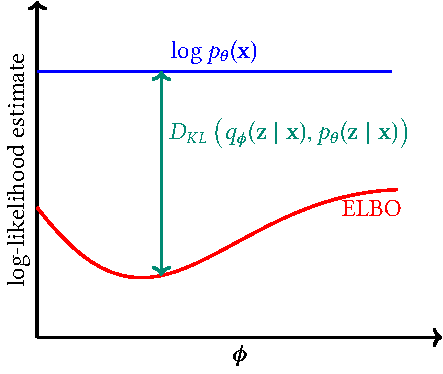
\includegraphics[width=0.5\linewidth]{Chapter2/Figs/Vector/elbo_diagram.pdf}
	\caption{ELBO is a lower bound of the log likelihood, the difference between the two is the KL divergence. The better the approximation of the posterior $q_{\boldsymbol{\phi}}(\mathbf{z}|\mathbf{x})$, the smaller is KL and consequently the closer is ELBO to $\log p_{\boldsymbol{\theta}}(\mathbf{x})$.}
	\label{fig:elbodiagram}
\end{figure}

\subsection{Variance Loss}
The evidence lower bound (ELBO) pathwise gradient estimator (SGVB), described in section~\ref{app:grad_estim}, has found great success but is limited to models with continuous latent variables. It would be more convenient to have a loss function that would deal with both discrete and continuous latent variables within the same framework. Recent work by Richter et al.~\cite{richter2020vargrad} analysed a score-function gradient estimator for ELBO and showed that it can be obtained from a different divergence measure, which they termed the \emph{log-variance loss}
\begin{equation}
	\mathcal{L}_{\text{LV}}\left(q_{\boldsymbol{\phi}}(\mathbf{z}) \| p_{\boldsymbol{\theta}}(\mathbf{z} \mid \mathbf{x})\right)=\frac{1}{2} \underset{\mathbf{\mathbf{z}} \sim r(\mathbf{\mathbf{z}})}{\operatorname{\mathbb{V}ar}}\left[\log \left(\frac{q_{\boldsymbol{\phi}}(\mathbf{z})}{p_{\boldsymbol{\theta}}(\mathbf{z} \mid \mathbf{x})}\right)\right],
\end{equation}
where $r(\mathbf{z})$ is some arbitrary distribution. Moreover, they showed that the gradient of $\mathcal{L}_{\text{LV}}$ w.r.t $\boldsymbol{\phi}$ corresponds to that of the KL divergence if $r(\mathbf{\mathbf{z}}) = q_{\boldsymbol{\phi}}(\mathrm{z})$ and provided a gradient estimator of the log-variance, thus suggested an optimisation procedure that works for both discrete and continuous latent distributions. In this work we will proceed in a similar fashion but with a different loss function. Motivated by the fact that when the posterior $q(z | x) = p(z | x)$ is exact we have
\begin{equation}
	\frac{p(\mathbf{x} \mid \mathbf{z}) p(\mathbf{z})}{q(\mathbf{z} \mid \mathbf{x})}=p(\mathbf{x}).
\end{equation}
The variance of $p(\mathbf{x})$ with regards to samples drawn from an arbitrary probability distribution $r(\mathbf{z})$ is zero which suggests the variance of the left hand side
\begin{equation}
	\mathcal{L}_{\boldsymbol{\phi}, \boldsymbol{\theta}}(\mathbf{x}) = \underset{\mathbf{z} \sim r(\mathbf{z})}{\operatorname{\mathbb{V}ar}}\left[\log \left(\frac{p_{\boldsymbol{\theta}}(\mathbf{x} \mid \mathbf{z}) p(\mathbf{z})}{q_{\boldsymbol{\phi}}(\mathbf{z} \mid \mathbf{x})}\right)\right]
\end{equation}
as an objective function. We can estimate the loss with sample variance using $S$ Monte Carlo samples
\begin{equation}
	\label{eq:varloss}
	\begin{aligned}
		\mathcal{L}_{\boldsymbol{\phi}, \boldsymbol{\theta}}(\mathbf{x}) \approx \frac{1}{(S-1)} &\sum_{s=1}^{S}\left(f_{\boldsymbol{\phi},\boldsymbol{\theta}}(\mathbf{z}^{(s)}, \mathbf{x})-\bar{f}_{\boldsymbol{\phi},\boldsymbol{\theta}}(\mathbf{x})\right)^{2}, \\
		\quad \mathbf{z}^{(s)} &\stackrel{\text { i.i.d. }}{\sim} r(\mathbf{z}),
	\end{aligned}
\end{equation}
where
\begin{equation}
	f_{\boldsymbol{\phi},\boldsymbol{\theta}} = \log \left(\frac{p_{\boldsymbol{\theta}}(\mathbf{x} \mid \mathbf{z}) p(\mathbf{z})}{q_{\boldsymbol{\phi}}(\mathbf{z} \mid \mathbf{x})}\right)
\end{equation}
and $f_{\boldsymbol{\phi},\boldsymbol{\theta}}$ is the average
\begin{equation}
	\bar{f}_{\boldsymbol{\phi},\boldsymbol{\theta}}(\mathbf{x})=\frac{1}{S} \sum_{s=1}^{S} f_{\boldsymbol{\phi},\boldsymbol{\theta}}\left(\mathbf{z}^{(s)},  \mathbf{x}\right).
\end{equation}
The gradient of expression~\eqref{eq:varloss} can be computed using automatic differentiation without any issue. The form of the gradient estimator of $\mathcal{L}_{\boldsymbol{\phi}, \boldsymbol{\theta}}(\mathbf{x})$ outlined above, is the same as the leave-one-out estimator described in~\cite{richter2020vargrad}, which means that it is an unbiased estimator of the gradient. The procedure of calculating the gradients for a given example $\mathbf{x}$ and parameters $\boldsymbol{\phi}, \boldsymbol{\theta}$ is given in Algorithm~\ref{alg:vargradEst}.
\begin{algorithm}[ht]
	\SetAlgoLined
	\KwIn{Encoder parameters $\boldsymbol{\phi}$, decoder parameters $\boldsymbol{\theta}$, example $\mathbf{x}$}
	\KwResult{Gradients w.r.t $\boldsymbol{\phi}, \boldsymbol{\theta}$ of the objective function $1$}
	\For{s = 1, \ldots, S}{
		$\boldsymbol{z}^{(s)} \leftarrow \operatorname{sample}\left(q_{\boldsymbol{\phi}}(\cdot \mid \mathbf{x})\right)$ \\
		$\boldsymbol{z}^{(s)} \leftarrow \operatorname{ stop\_gradient }\left(\boldsymbol{z}^{(s)}\right)$ \\
		$f_{\boldsymbol{\phi}, \boldsymbol{\theta}}^{(s)} \leftarrow \log p_{\boldsymbol{\theta}}(\boldsymbol{x} | \boldsymbol{z}^{(s)})p(\boldsymbol{z^{(s)}}) - \log q_{\boldsymbol{\phi}}(\mathbf{z}^{(s)} | \mathbf{x})$
	}
	$\widehat{\mathcal{L}} \leftarrow \text { Variance }\left(\left\{f_{\boldsymbol{\phi}, \boldsymbol{\theta}}^{(s)}\right\}_{s=1}^{S}\right)$ \\
	
	\Return $\operatorname{grad}\left(\widehat{\mathcal{L}}\right)$
	\caption{\label{alg:vargradEst}Gradients of $\mathcal{L}_{\boldsymbol{\boldsymbol{\phi}}, \boldsymbol{\theta}}(\mathbf{x})$}
\end{algorithm}
Importantly the samples $\mathbf{z}^{(s)}$, which will be for simplicity sampled from the model probability $\mathbf{z} \sim  q_{\boldsymbol{\phi}}(\mathbf{z} \mid \mathbf{x})$, must be detached from the computational graph so that backpropagation is possible. 

To test the applicability of the loss function we will test two variational autoencoders, one with continuous latent space and one with discrete latent space. The architecture of the neural networks that were used to parameterise the encoder and decoder will be discussed in chapter~\ref{chapter3}.

\subsection{Convolutional Neural Networks}


